\documentclass[12pt]{article}
\usepackage{url,graphicx,tabularx,array,geometry,amsmath,amssymb,amsthm,bbm,textcomp,algorithm}
\usepackage[noend]{algpseudocode}
\usepackage{nips12submit_e,times}
%\usepackage[sc]{mathpazo}

\newcommand{\unionf}{\bigcup_{n=1}^{\infty} \mathcal{F}_n}
\newcommand{\F}{\mathcal{F}}
\newcommand{\E}{\mathbb{E}}
\newcommand{\PP}{\mathbb{P}}
\newcommand{\Hi}{\mathcal{H}}
\newcommand{\A}{\mathcal{A}}
\newcommand{\Aseq}{\{A_k\}_{k=1}^{\infty}}
\newcommand{\unionA}{\bigcup_{k=1}^{\infty} A_k}
\newcommand{\argmax}{\operatornamewithlimits{argmax}}

\newenvironment{dedication}
        {\vspace{0.0ex}\begin{quotation}\begin{center}\begin{em}}
        {\par\end{em}\end{center}\end{quotation}}

\makeatletter
\def\BState{\State\hskip-\ALG@thistlm}
\makeatother

\nipsfinalcopy 

\begin{document}

\title{Segmenting Multivariate Time Series with Inertial Hidden Markov Models}

%...............................................................................
%                                   Authors
%...............................................................................
\author{
George D. Monta\~nez \\
Machine Learning Department\\
Carnegie Mellon University\\
Pittsburgh, PA USA\\
\texttt{gmontane@cs.cmu.edu} \\
\And    
Saeed Amizadeh\\
Media Sciences, Yahoo! Labs\\
Yahoo!\\
Sunnyvale, CA USA\\
\texttt{amizadeh@yahoo-inc.com} \\
\And
Nikolay Laptev \\
Media Sciences, Yahoo! Labs\\
Yahoo!\\
Sunnyvale, CA USA\\
\texttt{nlaptev@yahoo-inc.com} \\
}

\maketitle

\begin{abstract}
    Faced with the problem of segmenting a multivariate time series in an unsupervised manner, we derive and test two methods of regularizing hidden Markov models for this task. Regularization on state transitions provide smooth transitioning among states, such that the sequences are split into broad, contiguous segments. Our methods are compared with a recent hierarchical Dirichlet process hidden Markov model (HDP-HMM) and a baseline standard hidden Markov model, of which the former suffers from poor performance on moderate-dimensional data and sensitivity to parameter settings, while the latter suffers from rapid state transitioning, over-segmentation and poor performance on a segmentation task involving human activity accelerometer data from the UCI Machine Learning Repository. The regularized methods developed here are able to perfectly segment the human activity data in roughly half of the real-data test cases, with accuracy of 94\% and low variation of information. In contrast to the HDP-HMM, our methods provide simple, drop-in replacements for standard hidden Markov model update rules, allowing standard expectation maximization (EM) algorithms to be used for learning. Lastly, we make progress towards tuning the regularization strength in an unsupervised manner and derive equations for online learning of the regularized HMM parameters.
\end{abstract}

\section{Introduction}
\begin{dedication} ``Some seek complex solutions to simple problems; it is better to find simple solutions to complex problems.'' - \emph{Soramichi Akiyama}
\end{dedication}

This is where the introduction goes.


\section{Problem Statement}

Let $\mathbf{X} = \{\mathbf{x}_1, \ldots, \mathbf{x}_T\}$ denote a $d$-dimensional multivariate time series, where $\mathbf{x}_t \in \mathbb{R}^d$. Given such a time series, we seek to segment $\mathbf{X}$ along the time axis into \emph{segments}, where each segment corresponds to a subsequence $\mathbf{X}_{i\ldots i+m} = \{\mathbf{x}_i, \ldots, \mathbf{x}_{i+m}\}$ and maps to a predictive (latent) state $\mathbf{z}$, represented as a one-of-$K$ vector, where $|\mathbf{z}| = K$ and $\sum_{i=1}^{K}z_{t,i} = 1$. For simplicity of notation, let $\mathbf{z}_{t} = k$ denote $z_{t,k} = 1$ and let $\mathbf{Z} = \{\mathbf{z}_1, \ldots, \mathbf{z}_T\}$ denote the sequence of latent states. Then for all $\mathbf{x}_{t}$ mapping to state $k$, we require that
\begin{align*}
    \Pr(\mathbf{x}_{t+1}|\mathbf{X}_{1\ldots t}, \mathbf{z}_t = k) &= \Pr(\mathbf{x}_{t+1}| \mathbf{z}_t = k) \\
                                                                   &= \Pr(\mathbf{x}_{t'+1}| \mathbf{z}_{t'} = k) \\
                                                                   &= \Pr(\mathbf{x}_{t'+1}| \mathbf{X}_{1\ldots t'}, \mathbf{z}_{t'} = k).
\end{align*}
Thus, the conditional distribution over futures at time $t$ conditioned on being in state $k$ is equal to the distribution over futures at time $t'$ conditioned on being in the same state. Thus, we assume conditional independence given state, and stationarity of the generative process.

We impose two additional complexity criteria on our model. First, we seek models with a small number of latent states, $K \ll T$, and second, we desire state transition sequences of low complexity such that the transitioning of states does not occur too rapidly. We refer to this as the \emph{inertial transition} requirement, alluding to the physical property of matter that ensures it will continue along a fixed course unless acted upon by an external force. 

The above desiderata must be externally imposed on our model, since simply maximizing the likelihood of the data will result in $K = T$ (i.e., each sample corresponds a unique state/distribution), and in general we may have rapid transitions among states. For the first desideratum,  we choose the number of states in advance as is typically done for hidden Markov models~\cite{rabiner1989tutorial}. For the second, we directly alter the probabilistic form of our model to include a parameterized regularization that reduces the likelihood of transitioning between different latent states, encouraging state-persistence.

We next discuss the input and output for our problem setup.

\subsection{Problem Input}

As stated above, we are given a single $d$-dimensional multivariate time series of $T$ time samples. Alternatively, the single time series can be thought of as a collection of $d$ one-dimensional time series. As the generative story, we assume that at each time step $t$ a state $\mathbf{z}_t$ is chosen, given the previous state $\mathbf{z}_{t-1}$, according to the transition probabilities governing states. A $d$-dimensional point-sample is then drawn according to the emission density for state $\mathbf{z}_t$, and the process repeats for $1 < t \leq T$.

\subsection{Problem Output}

The output of the process is a list of integer tuples $(t, k)$, where $1 \leq t \leq T$ denotes the ending time of the segment and $1 \leq k \leq K$ the state that occurs during that segment. 

\section{Method}

\subsection{Inertial Hidden Markov Models}

Hidden Markov models~\cite{rabiner1989tutorial} (HMMs) are a class of long-studied probabilistic models well-suited for sequential data. As a starting point for developing our inertial HMMs, we begin a standard $K$-state HMM with Gaussian emission densities. HMMs (locally) maximize the likelihood of the data, but typically do not guarantee slow inertial transitioning among states. The number of states must be specified in advance, but no other parameters need to be given, as the remaining model parameters are all estimated directly from the data. 

To accommodate the inertial transition requirement, we derive two different methods of enforcing state-persistence in HMMs. Both methods alter the probabilistic form of the complete data joint likelihood function, which result in altered transition matrix update equations. The resulting update equations share a related mathematical structure and, as is shown in Section~\ref{sec:Results}, have similar performance on the datasets tested. 

We will next describe both methods and provide outlines of their derivations, with more detail being given to the derivation for the second method (the pseudo-observation inertial HMM).

\subsection{Maximum A Posteriori (MAP) Regularized HMM}

Following~\cite{MAP1994}, we alter the standard HMM to include a Dirichlet prior on the transition probability matrix, such that transitions out-of-state are penalized by some regularization factor. A Dirichlet prior on the transition matrix $\mathbf{A}$, for the $j$th row, has the form
\begin{align*}
    p(A_j; \eta) &\propto \prod_{i=1}^{K} A_{jk}^{\eta_{jk}-1}
\end{align*}
where the $\eta_{jk}$ are free parameters and $A_{jk}$ is the transition probability from state $j$ to state $k$. The posterior joint density over $\mathbf{X}$ and $\mathbf{Z}$ becomes
\begin{align*}
    P(\mathbf{X}, \mathbf{Z} ; \mathbf{\theta}, \eta) 
    &\propto \left[\prod_{i=1}^{K}\prod_{i=1}^{K} A_{jk}^{\eta_{jk} - 1}\right] P(\mathbf{X}, \mathbf{Z} \mid \mathbf{A}; \mathbf{\theta}) 
\end{align*}
and the log-likelihood is
\begin{align*}
\ell(\mathbf{X}, \mathbf{Z} ; \mathbf{\theta}, \eta) 
&\propto \sum_{i=1}^{K}\sum_{i=1}^{K} (\eta_{jk} - 1)\log A_{jk} + \log P(\mathbf{z}_{1}; \theta) + \sum_{t=1}^{T}\log P(\mathbf{x}_t|\mathbf{z}_t; \mathbf{\theta}) + \sum_{t=2}^{T}\log P(\mathbf{z}_t|\mathbf{z}_{t-1}; \mathbf{\theta}).
\end{align*}

MAP estimation is then used in the M-step of the EM algorithm, to update the transition probability matrix. Maximizing, with appropriate Lagrange multiplier constraints, we obtain the update equation for the transition matrix, 
\begin{align}
    A_{jk} &= \frac{(\eta_{jk} - 1) + \sum_{t=2}^{T} \xi(z_{(t-1)j}, z_{tk})}   
    {\sum_{i=1}^{K}(\eta_{ji} - 1) + \sum_{i=1}^{K}\sum_{t=2}^{T} \xi(z_{(t-1)j}, z_{ti})}.
\end{align}

Given our prior, we can control the probability of self-transitions among states, but this method requires that we choose a set of $K^2$ parameters for the Dirichlet prior. However, since we are solely concerned about increasing the probability of self-transitions, we can reduce these parameters to a single parameter $\lambda$ governing the amplification of self-transitions. We therefore define $\eta_{jk} = 1$ when $j\not=k$ and $\eta_{kk}= \lambda \geq 1$ otherwise, and the transition update equation becomes
\begin{align}\label{eq:MAP-final}
    A_{jk} &= \frac{(\lambda - 1){\mathbbm{1}(j = k)} + \sum_{t=2}^{T} \xi(z_{(t-1)j}, z_{tk})}   
    {(\lambda - 1) + \sum_{i=1}^{K}\sum_{t=2}^{T} \xi(z_{(t-1)j}, z_{ti})}
\end{align}
where $\mathbbm{1}(\cdot)$ denotes the indicator function.

\subsubsection{Inertial Regularization via Pseudo-observations}

We now derive a second method of regularizing the state transitions, where we alter the HMM likelihood function to include a fictional observation, $V$. This is a binary random variable indicating that a transition was chosen at random from among all transitions, according to some distribution, and that the transition observed was a self-transition. Thus, we view the transitions as being partitioned into two sets, self-transitions and non-self-transitions, and we draw a member of the self-transition set according to a Bernoulli distribution governed by some parameter $p$. Given a latent state sequence $\mathbf{Z}$, with transitions chosen according to transition matrix $\mathbf{A}$, we define $p$ as a function of both $\mathbf{Z}$ and $\mathbf{A}$. We would like $p$ to have two properties: 1) it should increase with increasing $\sum_k A_{kk}$ (probability of self-transitions) and 2) it should increase as the number of self-transitions in $\mathbf{Z}$ increases. This will allow us to encourage self-transitions as a simple consequence of maximizing the likelihood of our observations.

We begin with a version of $p$ based on a penalization constant $0 < \epsilon < 1$ that scales appropriately with the number of self-transitions. If we raise $\epsilon$ to a large positive power, the resulting $p$ will decrease. Thus, we define $p$ as $\epsilon$ raised to the number of non-self-transitions in the state transition sequence, so that the probability of selecting a self-transition increases as the number of non-self-transitions decreases. Using the fact that the number of non-self-transitions equals $(T-1) - \sum^{T}_{t=2}\sum^{K}_{k=1}z_{(t-1)k}z_{tk}$, we obtain 
\begin{align}
    p &= \epsilon^\text{\tiny NUM.\ OF NON-SELF-TRANSITIONS}\\
      &= \epsilon^{(T-1) - \sum^{T}_{t=2}\sum^{K}_{k=1}z_{(t-1)k}z_{tk}} \notag\\
      &= \epsilon^{\sum^{T}_{t=2}1 - \sum^{T}_{t=2}\sum^{K}_{k=1}z_{(t-1)k}z_{tk}} \notag\\
      &= \epsilon^{\sum^{T}_{t=2}\sum^{K}_{k=1}z_{(t-1)k} - \sum^{T}_{t=2}\sum^{K}_{k=1}z_{(t-1)k}z_{tk}} \notag\\
      &= \epsilon^{\sum^{T}_{t=2}\sum^{K}_{k=1}z_{(t-1)k} - z_{(t-1)k}z_{tk}} \notag\\
      &= \prod^{T}_{t=2}\prod_{k=1}^{K}\epsilon^{z_{(t-1)k} - z_{(t-1)k}z_{tk}}. \label{eq:eps-0}
\end{align}

Since $\epsilon$ is arbitrary, we choose $\epsilon = A_{kk}$, to allow $p$ to scale appropriately with increasing probability of self-transition. We therefore arrive at
\begin{align*}
    p &= \prod^{T}_{t=2}\prod^{K}_{k=1}A_{kk}^{z_{(t-1)k} - z_{(t-1)k}z_{tk}}.
\end{align*}
Thus, we define $p$ as a computable function of $\mathbf{Z}$ and $\mathbf{A}$. Defining $p$ in this deterministic manner is equivalent to choosing the parameter value from a degenerate probability distribution that places a single point mass at the value computed, allowing us to easily obtain a posterior distribution on $V$. Furthermore, we see that the function increases as the number of self-transitions increases, since $A_{kk} \leq 1$ for all $k$, and $p$ will generally increase as $\sum_k A_{kk}$ increases. Thus, we obtain a parameter $p \in (0,1]$ that satisfies all our desiderata.

With $p$ in hand, we say that $V$ is drawn according to the Bernoulli distribution, Bern($p$), and we observe $V = 1$ (i.e., a member of the self-transition set was chosen). Since $P(V = 1|\mathbf{Z};\mathbf{A}) = p$, we have
\begin{align*}
    P(V = 1|\mathbf{Z}; \mathbf{A}) &= \prod^{T}_{t=2}\prod^{K}_{k=1}A_{kk}^{z_{(t-1)k} - z_{(t-1)k}z_{tk}}.
\end{align*}
To gain greater control over the strength of regularization, let $\lambda$ be a positive integer and $\mathbf{V}$ be an $\lambda$-length sequence of pseudo-observations, drawn i.i.d.\ according to Bern($p$). Thus, 
\begin{align*}
    P(\mathbf{V} = \mathbf{1}|\mathbf{Z}; \mathbf{A}) &= \left[\prod^{T}_{t=2}\prod^{K}_{k=1}A_{kk}^{z_{(t-1)k} - z_{(t-1)k}z_{tk}}\right]^\lambda
\end{align*}
where $\mathbf{1}$ denotes the all-ones sequence of length $\lambda$.

Clearly $\mathbf{V}$ is conditionally independent of $\mathbf{X}$ given the latent state sequence $\mathbf{Z}$. We now consider the joint density over $\mathbf{X}$, $\mathbf{V}$, and $\mathbf{Z}$, making use of our conditional independence assumption. We parameterize the joint density by $\mathbf{\theta} = \{\mathbf{\pi},\mathbf{A}, \mathbf{\phi}\}$, which are the start-state probabilities, state transition matrix and emission parameters, respectively. We have
\begin{align*}
    P(\mathbf{X}, \mathbf{V}, \mathbf{Z} ; \mathbf{\theta}) 
    &= P(\mathbf{V}|\mathbf{Z}; \mathbf{\theta}) P(\mathbf{z}_{1} ; \theta) \left[\prod_{t=1}^{T}P(\mathbf{x}_t|\mathbf{z}_t; \mathbf{\theta})\right]\left[\prod_{t=2}^{T}P(\mathbf{z}_t|\mathbf{z}_{t-1}; \mathbf{\theta})\right]
\end{align*}
and, taking the log of the likelihood,
\begin{align*}
    \ell(\mathbf{X}, \mathbf{V}, \mathbf{Z} ; \mathbf{\theta}) 
    &= \log P(\mathbf{V}|\mathbf{Z}; \mathbf{\theta}) + \log P(\mathbf{z}_{1}; \theta) + \sum_{t=1}^{T}\log P(\mathbf{x}_t|\mathbf{z}_t; \mathbf{\theta}) + \sum_{t=2}^{T}\log P(\mathbf{z}_t|\mathbf{z}_{t-1};\mathbf{\theta}).
\end{align*}

Noting that 
\begin{align*}
    P(\mathbf{z}_{1}; \theta) &= \prod_{k=1}^{K}\pi_{k}^{z_{1k}}, \\
    P(\mathbf{x}_t|\mathbf{z}_t; \mathbf{\theta}) &= \prod_{k=1}^{K} P(\mathbf{x}_t ; \mathbf{\phi}_k)^{z_{tk}},\text{ and }\\ 
    P(\mathbf{z}_t|\mathbf{z}_{t-1}; \mathbf{\theta}) &= \prod_{k=1}^{K}\prod_{j=1}^{K}A_{jk}^{z_{(t-1)j}z_{tk}},
\end{align*}
and substituting into $\ell(\mathbf{X}, \mathbf{V}, \mathbf{Z} ; \mathbf{\theta})$ we obtain
\begin{align*}
    \ell(\mathbf{X}, \mathbf{V}=\mathbf{1}, \mathbf{Z} ; \mathbf{\theta}) 
    &= \sum^{T}_{t=2}\sum^{K}_{k=1}\lambda[z_{(t-1)k} - z_{(t-1)k}z_{tk}]\log A_{kk} + \sum_{k=1}^{K}{z_{1k}}\log \pi_{k} \notag\\
    &+ \sum_{t=1}^{T}\sum_{k=1}^{K} z_{tk}\log P(\mathbf{x}_t ; \mathbf{\phi}_k) + \sum_{t=2}^{T}\sum_{k=1}^{K}\sum_{j=1}^{K}[z_{(t-1)j}z_{tk}]\log A_{jk}.
\end{align*}

Following Bishop~\cite{bishop2007pattern}, we define
\begin{align*}
    \gamma(z_{tk}) &= \mathbb{E}[z_{tk}] = \sum_{\mathbf{z}}\gamma(\mathbf{z})z_{tk} \\
    \xi(z_{(t-1)j}, z_{tk}) &= \mathbb{E}[z_{(t-1)j}z_{tk}] = \sum_{\mathbf{z}}\gamma(\mathbf{z})z_{(t-1)j}z_{tk}
\end{align*}
to obtain
\begin{align}\label{eq:main}
    \mathbb{E}_{\mathbf{Z}}[\ell(\mathbf{X}, \mathbf{V}=\mathbf{1}, \mathbf{Z} ; \mathbf{\theta})]
    &= \sum^{T}_{t=2}\sum^{K}_{k=1}\lambda[\gamma(z_{(t-1)k})-\xi(z_{(t-1)k}, z_{tk})]\log A_{kk} + \sum_{k=1}^{K}\gamma(z_{1k})\log \pi_{k} \notag\\
    &+ \sum_{t=1}^{T}\sum_{k=1}^{K} \gamma(z_{tk})\log P(\mathbf{x}_t ; \mathbf{\phi}_k) + \sum_{t=2}^{T}\sum_{k=1}^{K}\sum_{j=1}^{K}\xi(z_{(t-1)j}, z_{tk})\log A_{jk}.
\end{align}

Using Lagrange multipliers, taking the derivative of (\ref{eq:main}) with respect to $A_{jk}$ and setting to the result to zero, we obtain the regularized maximum likelihood estimate for $A_{jk}$, namely
\begin{align*}
    A_{jk} &= \frac{\sum_{t=2}^{T} \xi(z_{(t-1)k}, z_{tk}) + \sum_{t=2}^{T}{\mathbbm{1}(j = k)}\lambda[\gamma(z_{(t-1)k}) - \xi(z_{(t-1)k}, z_{tk})]}   
    { \sum_{t=2}^{T} \sum_{i=1}^{K} \left(\xi(z_{(t-1)j}, z_{ti}) + {\mathbbm{1}(j = i)}\lambda[\gamma(z_{(t-1)i}) - \xi(z_{(t-1)i}, z_{ti})]\right)}
\end{align*}
where $\mathbbm{1}(\cdot)$ denotes the indicator function. The forward-backward algorithm can then be used for efficient computation of the $\gamma$ and $\xi$ values, as is the case for unregularized HMMs.

Ignoring normalization, we see that
\begin{align*}
    A_{jk} &\propto \begin{cases} 
                \sum_{t=2}^{T} \xi(z_{(t-1)k}, z_{tk}) + \lambda\sum_{t=2}^{T}[\gamma(z_{(t-1)k}) - \xi(z_{(t-1)k}, z_{tk})] & \mbox{if } j=k \\ 
                \sum_{t=2}^{T} \xi(z_{(t-1)j}, z_{tk}) & \mbox{otherwise.}
              \end{cases}
\end{align*}
Thus, $\lambda$ is a multiplier of additional mass contributions for self-transitions, where the contributions are the difference between $\gamma(z_{(t-1)k})$ and $\xi(z_{(t-1)k}, z_{tk})$. These two quantities represent, respectively, the expectation of being in a state $k$ at time $t-1$ and the expectation of remaining there in the next time step. The larger $\lambda$ or the larger the difference between arriving at a state and remaining there, the greater the additional mass given to self-transition. 

Similar to the MAP case, we let $\lambda = (T-1)^{\zeta}$ to maintain consistent regularization strength in the face of increasing sequence length, where $\zeta$ becomes our new regularization parameter.


\subsubsection{Scale-Free Regularization}

In Equation~\ref{eq:MAP-final}, the strength of the regularization diminishes with growing $T$, so that asymptotically the regularized estimate and unregularized estimate become equivalent. While this is often desirable in other contexts, maintaining a consistent strength of inertial regularization becomes important with time series of increasing length, as is the case with online learning methods. Figure~\ref{fig:short-real-data} shows a regularized segmentation of human accelerometer data (discussed later in the Experiments section), where the regularization is strong enough to correctly segment the series into large, contiguous sections. If we then increase the number of data points in each section by a factor of ten while keeping the same regularization parameter setting, we see that the regularization is no longer strong enough, as is shown in Figure~\ref{fig:long-real-data}. Two of the sections have become splintered into small, choppy regions. Thus, the $\lambda$ parameter is sensitive to the size of the time series.

\begin{figure}[htbp]
  \caption{Human activities accelerometer data, short sequence. Vertical partitions correspond to changes of state. Only one dimension of data is shown.}
  \centering
    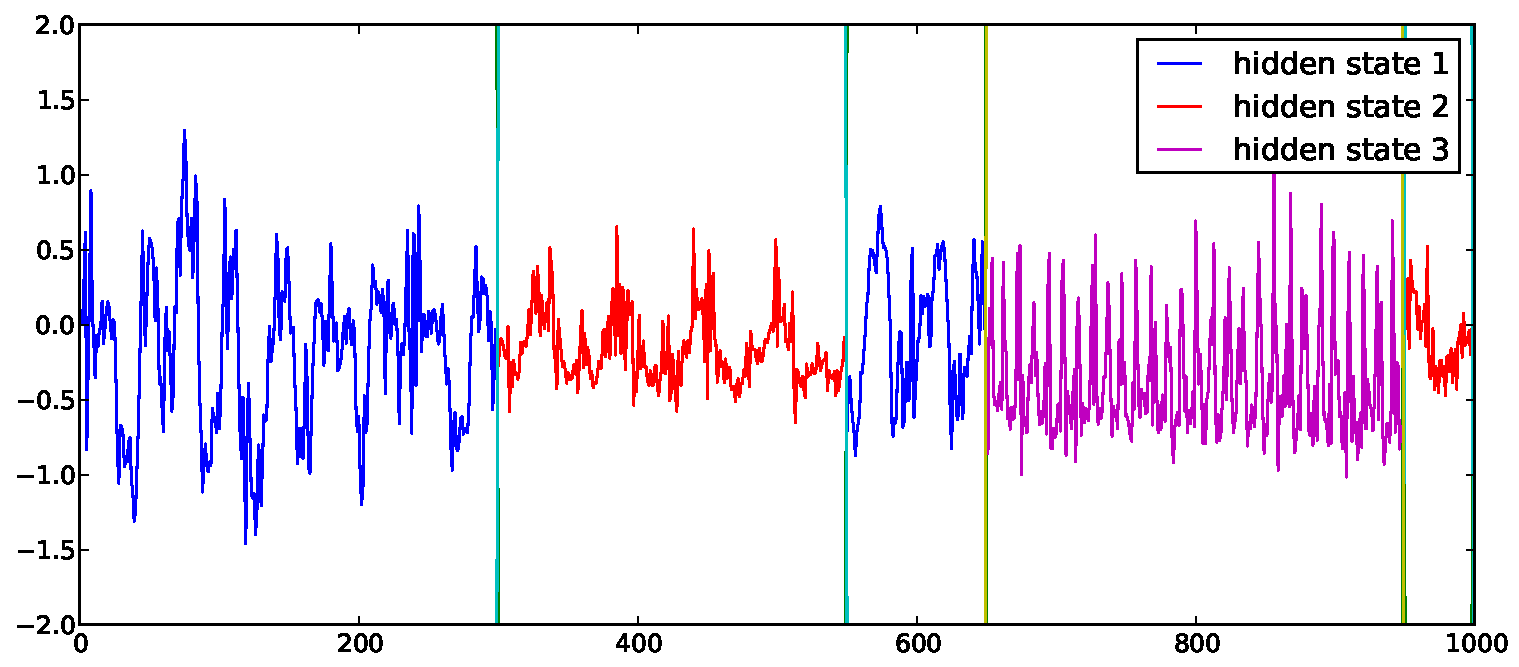
\includegraphics[width=0.8\linewidth]{images/MAP_results_hard_activity_short_3_states.pdf}
    \label{fig:short-real-data}
\end{figure}

\begin{figure}[htbp]
  \caption{Human activities accelerometer data, long sequence. Regularization parameter from short sequence used here.}
  \centering
    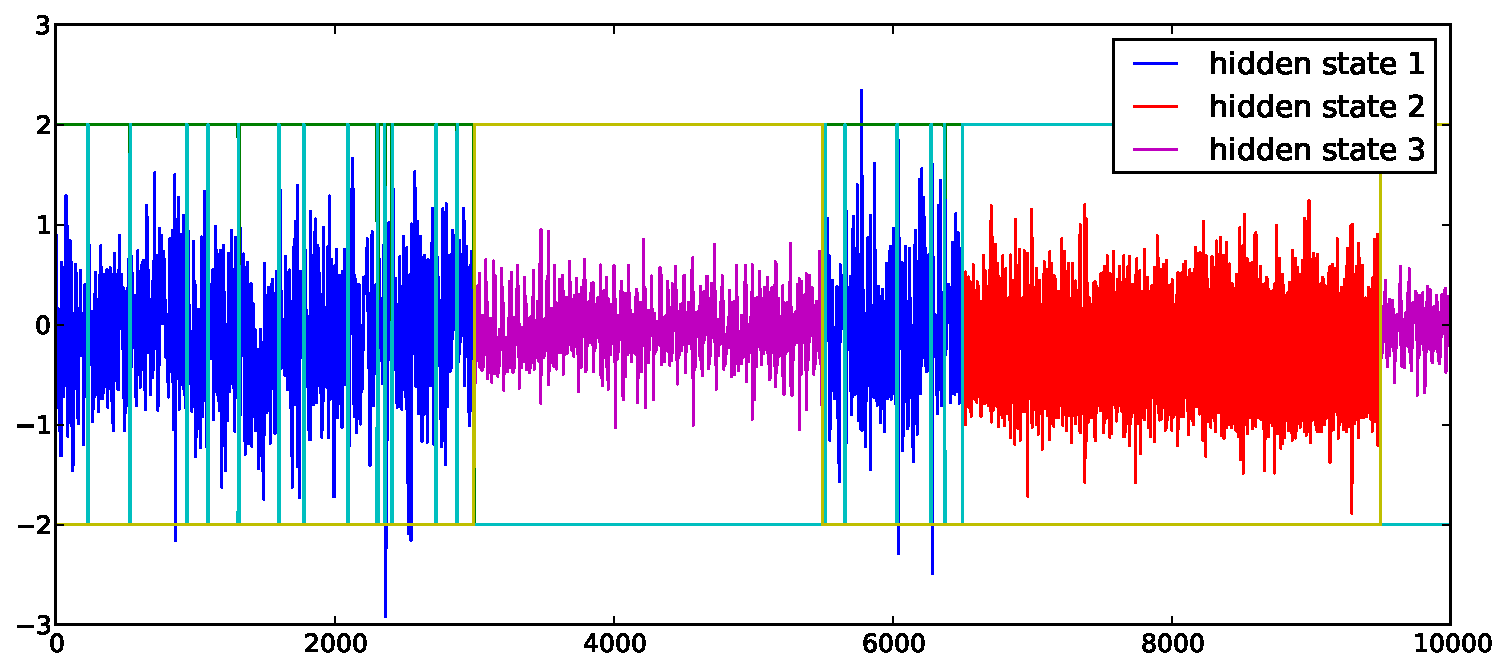
\includegraphics[width=0.8\linewidth]{images/MAP_results_hard_activity_long_3_states.pdf}
    \label{fig:long-real-data}
\end{figure}

We desire models where the regularization strength is scale-free, having roughly the same strength regardless of how the time series grows. To achieve this, we define the $\lambda$ parameter to scale with the number of transitions, namely $\lambda = (T-1)^\zeta$, and our scale-free update equation becomes
\begin{align}\label{eq:SCALE-FREE-MAP}
    A_{jk} &= \frac{((T - 1)^{\zeta}-1){\mathbbm{1}(j = k)} + \sum_{t=2}^{T} \xi(z_{(t-1)j}, z_{tk})}   
    {((T - 1)^{\zeta} - 1) + \sum_{i=1}^{K}\sum_{t=2}^{T} \xi(z_{(t-1)j}, z_{ti})}.
\end{align}
This preserves the effect of regularization as $T$ increases, and $\zeta$ becomes our new regularization parameter, controlling the strength of the regularization. For consistency, we also re-parameterize Equation~\ref{eq:PSO-final} using the same form, i.e., $\lambda = (T-1)^\zeta$.

%Figures~\ref{fig:short-real-data-scale-free} and \ref{fig:long-real-data-scale-free} shows the scale-free regularized result on both a short and long sequence, using the same regularization parameter. The parameter was chosen in reference to the short sequence, selecting the smallest parameter that still provided correct segmentation. As can be seen, the regularization strength is sufficient for the long sequence as well, illustrating the effectiveness of a scale-free parameterization.
%
%\begin{figure}[htbp]
%  \caption{Human activities accelerometer data, short sequence, with minimum scale-free regularization parameter.}
%  \centering
%    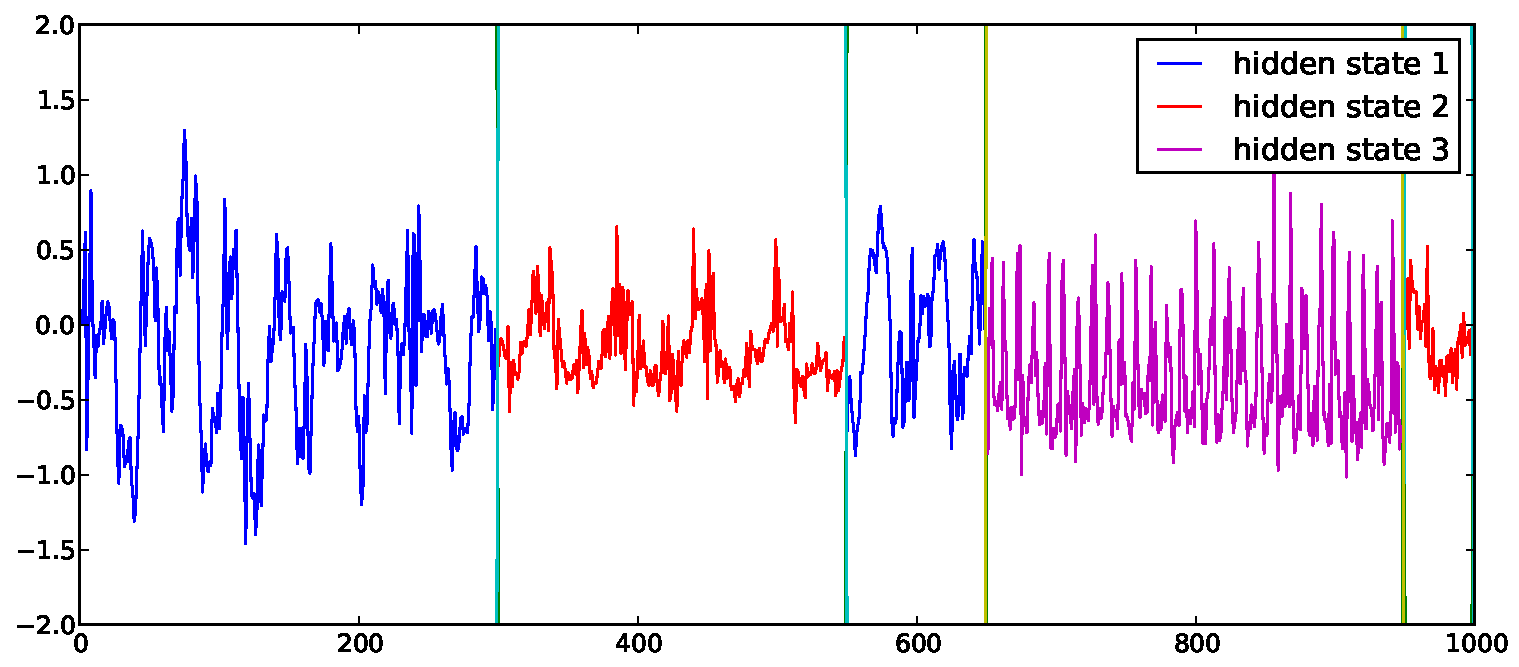
\includegraphics[width=.8\linewidth]{images/MAP_SCALE_FREE_results_hard_activity_short_3_states.pdf}
%    \label{fig:short-real-data-scale-free}
%\end{figure}
%
%\begin{figure}[htbp]
%  \caption{Human activities accelerometer data, long sequence, with minimum scale-free regularization parameter chosen in regards to short sequence. Correct segmentation is maintained despite the length of the time series increasing by an order of magnitude.}
%  \centering
%    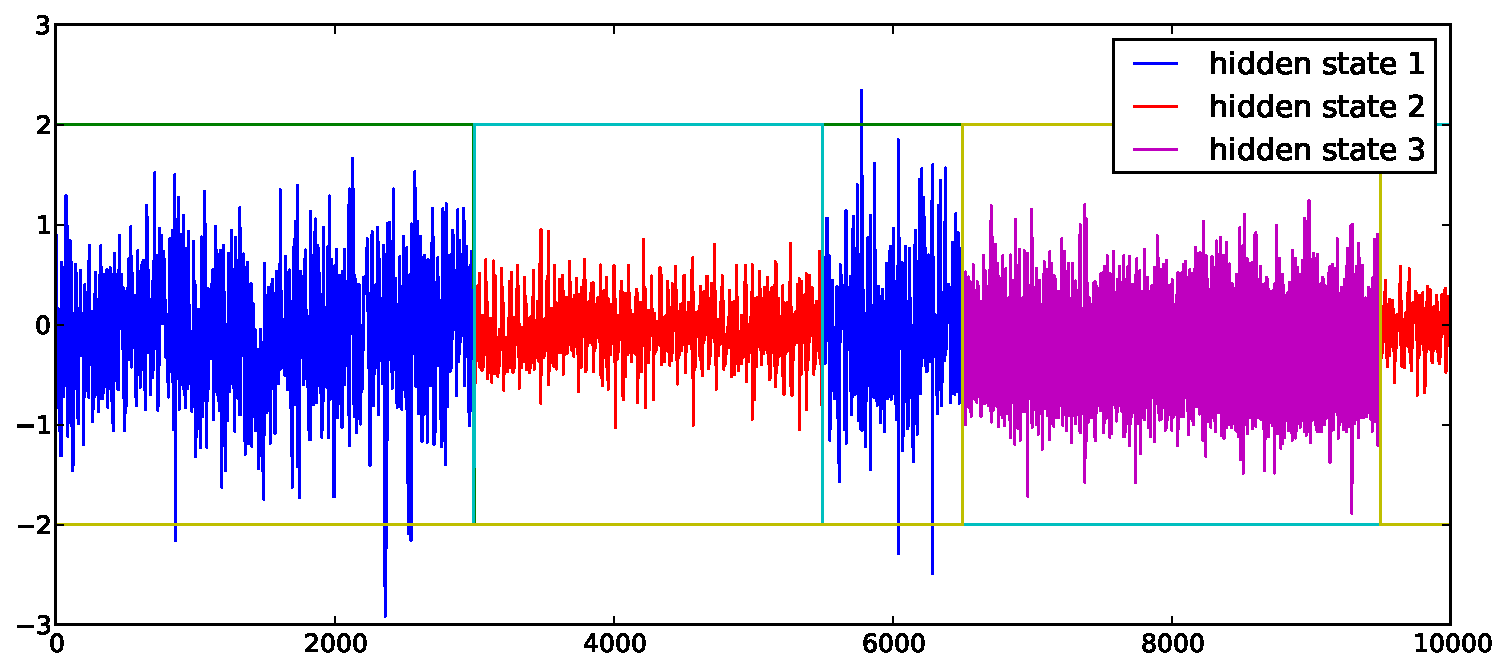
\includegraphics[width=.8\linewidth]{images/MAP_SCALE_FREE_results_hard_activity_long_3_states.pdf}
%    \label{fig:long-real-data-scale-free}
%\end{figure}

\subsubsection{Towards Parameter-Free Regularization}\label{sec:param-free}

The two methods of inertial transition regularization work well as long as the strength of regularization is provided. Here we seek to develop a version of the regularized HMM that does not require specification in advance of the regularization parameter. We accomplish this by making an assumption concerning the distribution of segment lengths. If we assume that most of the segment lengths are of roughly the same order-of-magnitude scale, then for a fixed $K$, we can automatically tune the regularization parameter.

We first define a range of possible regularization parameter values (such as $\lambda \in [0, 75]$), and perform a search on this interval for a value that gives sufficient regularization. ``Sufficient regularization'' is defined with regards to the Gini ratio~\cite{gini1936,wiki:1}, which is a measure of statistical dispersion often used to quantify income inequality. For a collection of observed segment lengths $L = \{l_1, \ldots, l_m\}$, given in ascending order, the Gini ratio is estimated by
\begin{align*}
    G(L) &= 1 - \frac{2}{m-1}\left(m - \frac{\sum_{i=1}^{m} i l_i}{\sum_{i=1}^{m} l_i}\right).
\end{align*}

Our assumption is that the true segmentation has a Gini ratio less than one-half, which corresponds to having more equality among segment lengths than not. One can perform a binary search on the search interval to find the smallest $\zeta$ parameter for which the Gini ratio is at least one-half. This incurs a computation cost of increasing time complexity by a factor of $O(\log_2 (R / \epsilon))$, where $R$ is the range of the parameter space.

\subsection{Online Learning of Inertial HMM parameters}

Hidden Markov models traditionally use batch methods for learning model parameters, such as Baum-Welch EM. Since our inertial regularization methods rely on standard EM learning, we can naturally incorporate incremental EM learning techniques into our system. We thus extend the work of Stenger \emph{et al.}~\cite{stenger2001} to provide an online learning algorithm for our regularized MAP hidden Markov model, which allows scaling to arbitrarily large datasets. Theoretical justification for incremental online EM learning is given in~\cite{Neal:1999:VEA:308574.308679}.

\subsubsection{Parameter Update Equations}

Define $D_{T,i} := ((T-1)^\zeta -1) + \sum_{t=2}^{T}\sum_{k=1}^{K} \xi(z_{(t-1)i}, z_{tk})$. The recurrence for $D_{T,i}$ is
\begin{align*}
    D_{T,i} &= [(T-1)^\zeta - (T-2)^\zeta] +  \sum_{k=1}^{K} \xi(z_{(T-1)i}, z_{Tk}) + D_{(T-1), i}
\end{align*}
where $T$ is the current time-step. Since $T$ is both the current and final time-step, we have $\beta(z_{T,k}) = 1$ for $k = 1, \ldots, K$, and thus
\begin{align*}
    \xi(\mathbf{z}_{t-1}, \mathbf{z}_{t}) 
            &= P(\mathbf{z}_{t-1}, \mathbf{z}_{t} | \mathbf{X}) \\
            &= \frac{\alpha(\mathbf{z}_{t-1})p(\mathbf{x}_t|\mathbf{z}_t; \phi)p(\mathbf{z}_{t}|\mathbf{z}_{(t-1)})\beta(\mathbf{z}_t)}{p(\mathbf{X})} \\
            &= \frac{\alpha(z_{(t-1)i})p(\mathbf{x}_t; \phi_j)A_{ij}^{(T-1)}}{\sum_{k=1}^{K}\alpha(z_{tk})}
\end{align*}
where
\begin{align*}
    \alpha(z_{tj}) &= \left[\sum_{i=1}^{K} \alpha(z_{(t-1)i})A_{ij}^{(t-1)}\right]p(\mathbf{x}_t; \phi_j).
\end{align*}

An efficient online update equation for the regularized transition matrix is then given by
\begin{align*}
    A_{ij}^{(T)} &= \frac{\xi(z_{(T-1)i}, z_{Tj})}{D_{T,i}} + \frac{\mathbbm{1}(i = j)[(T-1)^\zeta - (T-2)^\zeta]}{D_{T,i}} + \frac{D_{(T-1), i}}{D_{T,i}}A_{ij}^{(T-1)}.
\end{align*}

Also, because $\beta(z_{T,k}) = 1$, we have $\gamma(z_{tk}) = \alpha(z_{tk}) / \sum_{i=1}^{K}\alpha(z_{ti})$. The corresponding incremental update equations for a Gaussian emission model (as reported in~\cite{stenger2001}) are 
\begin{align*}
    \mathbf{\mu}_{j}^{(T)} &= \frac{\sum_{t=1}^{T-1}\gamma(z_{tj})}{\sum_{t=1}^{T}\gamma(z_{tj})}\mathbf{\mu}_{j}^{(T-1)} + \frac{\gamma(z_{Tj})}{\sum_{t=1}^{T}\gamma(z_{tj})}\mathbf{x}_T
\end{align*}
and
\begin{align*}
    \mathbf{S}_j^{(T)} &= \frac{\sum_{t=1}^{T-1}\gamma(z_{tj})}{\sum_{t=1}^{T}\gamma(z_{tj})}\mathbf{S}_j^{(T-1)} + \frac{\gamma(z_{Tj})}{\sum_{t=1}^{T}\gamma(z_{tj})}\left(\mathbf{x}_T - \mathbf{\mu}_j^{(T)}\right)\left(\mathbf{x}_T - \mathbf{\mu}_j^{(T)}\right)'
\end{align*}
where $(\cdot)'$ denotes the matrix transpose operation and $\mathbf{S}_j$ is the covariance matrix for state $j$.

\subsubsection{Initialization}

The process begins by batch-learning initial parameter estimates from a small portion of the time-series. These estimates are used for $\mathbf{A}^{(1)}$, $\mathbf{\mu}^{(1)}$, $\mathbf{S}^{(1)}$ and $\pi(\mathbf{z}_t)$. For the $\alpha$ values, we initialize $\alpha(z_{1j}) = \pi(z_{1j})p(\mathbf{x}_1; \phi_j)$ for each $j$. Using Equation~\ref{eq:SCALE-FREE-MAP} and the definition of $D_{T,i}$, we compute
\begin{align*}
    D_{2,i} &= \sum_{j=1}^{K} \xi(z_{1i}, z_{2j}), \\
    A_{ij}^{(2)} &= \frac{\xi(z_{1i}, z_{2j})}{D_{2,i}}.
\end{align*}
The estimates are then updated for each new observation, using the update equations given above. Algorithm~\ref{alg:incremental} outlines the order in which the various terms are computed.

\begin{algorithm}
\caption{}
\begin{algorithmic}[1]
\Procedure{Incremental Learning of Regularized HMM}{}
\State Batch learn initial parameter estimates from short segment of data.
\State Compute $D_{2,i}$ and $A_{ij}^{(2)}$ for all $i,j$.
\BState For $T > 2$:
\State Compute $\alpha$ values for observation at time $T$.
\State Compute $\xi(z_{(T-1)i},z_{Tj})$ values for all $i,j$.
\State Compute $\gamma(z_{Tj})$ and $D_{T,i}$ values for all $i,j$.
\State Update $A_{i,j}^{(T)}$ using incremental update rule.
\State Update $\mathbf{\mu}_{j}^{(T)}$ and $\mathbf{S}_{j}^{(T)}$ using incremental update rules.
\EndProcedure
\end{algorithmic}
\label{alg:incremental}
\end{algorithm}

%\subsubsection{Robust Online Prediction}
%
%In keeping with our desire for slow state transitions, we now consider the problem of incremental prediction. If an observation at time $t$ (the current time step) is an outlier, we cannot know whether the model should remain in the same hidden state, treating the outlier as an anomaly, or transition to a new hidden state. To overcome this limitation, we propose delayed prediction of state labels using a sliding window of length $w$. As the window moves through the observation sequence, the Viterbi algorithm is performed on the section of data within the window and a prediction for the $(t - w/2)$th observation is output. This allows for ``future'' observations to affect ``past'' observations within the window, via the backtracking maximization performed by the algorithm. Assuming we batch-learned an initial segment of data longer than $w/2$, we can begin output delayed state label predictions as soon as incremental learning begins.
%
\section{Experiments}\label{sec:Experiments}

We perform two segmentation tasks on simulated and real multivariate time series data, using our scale- and parameter-free regularized inertial HMMs. For comparison, we present the results of applying a standard $K$-state hidden Markov model as well as the Bayesian hierarchical Dirichlet process hidden Markov model (sticky HDP-HMM) of Fox \emph{et al.}~\cite{fox2011sticky}. We performed all tasks in an unsupervised manner, with state labels being used only for evaluation.

\subsection{Data}\label{sec:datasets}

A simulated dataset was generated using a two-state HMM with 3-D Gaussian emissions, with transition matrix
\begin{align*}
    \mathbf{A} &= \left( 
                   \begin{array}{ccc}
                    0.9995 & 0.0005 \\
                    0.0005 & 0.9995
                   \end{array}
                   \right),
\end{align*}
equal start probabilities and emission parameters $\mathbf{\mu}_1 = (-1, -1, -1)^\top$, $\mathbf{\mu}_2 = (1, 1, 1)^\top$, $\mathbf{\Sigma}_1 = \mathbf{\Sigma}_2 = \text{diag}(3)$. Using this model, we generated one hundred time series consisting of ten-thousand time points each. Figure~\ref{fig:simulated} shows an example time series from this simulated dataset.

\begin{figure}[htbp]
  \caption{Simulated data example. Generated from two-state HMM with 3D Gaussian emissions and strong self-transition behavior.}
  \centering
    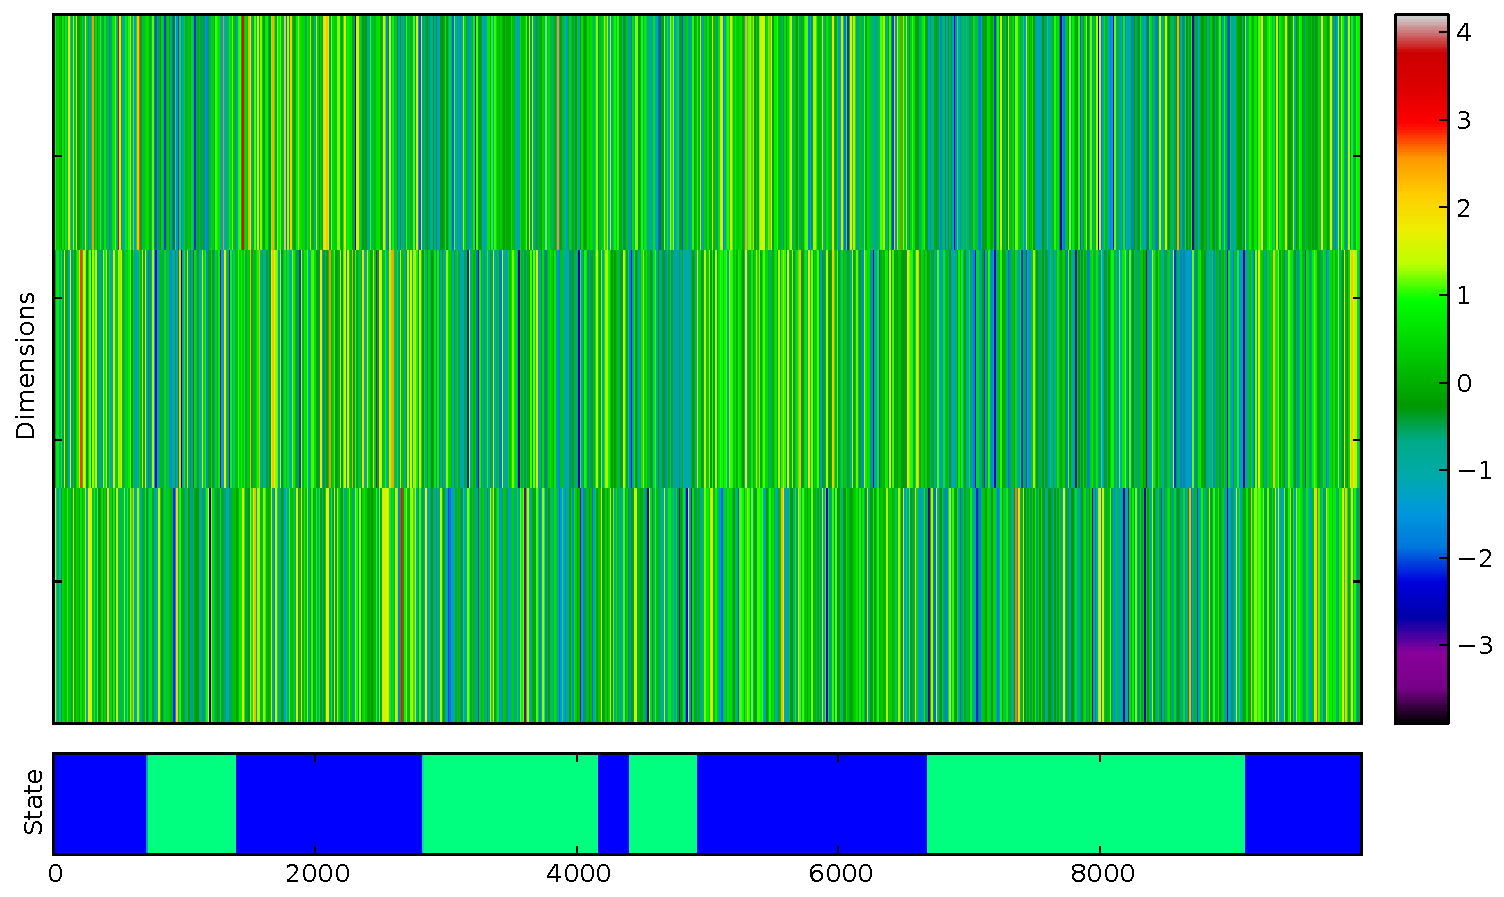
\includegraphics[width=1.\linewidth]{images/3D_synthetic_data_example.pdf}
    \label{fig:simulated}
\end{figure}
The second dataset is generated from real-world forty-five dimensional human accelerometer data~\cite{Altun:2010:CSC:1823245.1823314} recorded for users performing five different activities, namely, playing basketball, rowing, jumping, ascending stairs and walking in a parking lot. The data were recorded from a single subject using five Xsens MTx\texttrademark\ units attached to the torso, arms and legs. Each unit had nine sensors, which recorded accelerometer $(X, Y, Z)$ data, gyroscope $(X,Y,Z)$ data and magnetometer $(X,Y,Z)$ data, for a total of forty-five signals at each time point.

We generated one hundred multivariate times series from the underlying dataset, with varying activities (latent states) and number of segments. To generate these sets, the process was as follows. First, we uniformly chose the number of segments, between two and twenty. Then, for each segment, we chose an activity uniformly at random from among the five possible, and selected a uniformly random segment length proportion. The selected number of corresponding time points were extracted from the activity (keeping track of position in the sequence, and modulo the length of the sequence), rescaled to zero mean and unit variance, and appended to the output sequence. The final output sequence was truncated to ten thousand time points, or discarded if the sequence contained fewer than ten thousand points or fewer than two distinct activities. Additionally, prospective time series were rejected and replaced if they caused numerical instability issues for the algorithms tested, which occurred for some time series with many (or extremely short) segments. This process produced multivariate time series of fixed length, with varying number of segments, activities and segment lengths. The process was repeated to generate one hundred such time series of ten thousand time points each used in the quantitative analysis described in Section~\ref{sec:quantitative}. An example of such generated data sequences is shown in Figure~\ref{fig:accelerometer} and the distribution of the time series according to number of activities and segments is shown in Figure~\ref{fig:distribution}.

\begin{figure}[htbp]
  \caption{Human activities accelerometer data. Three state, 45-dimensional.}
  \centering
    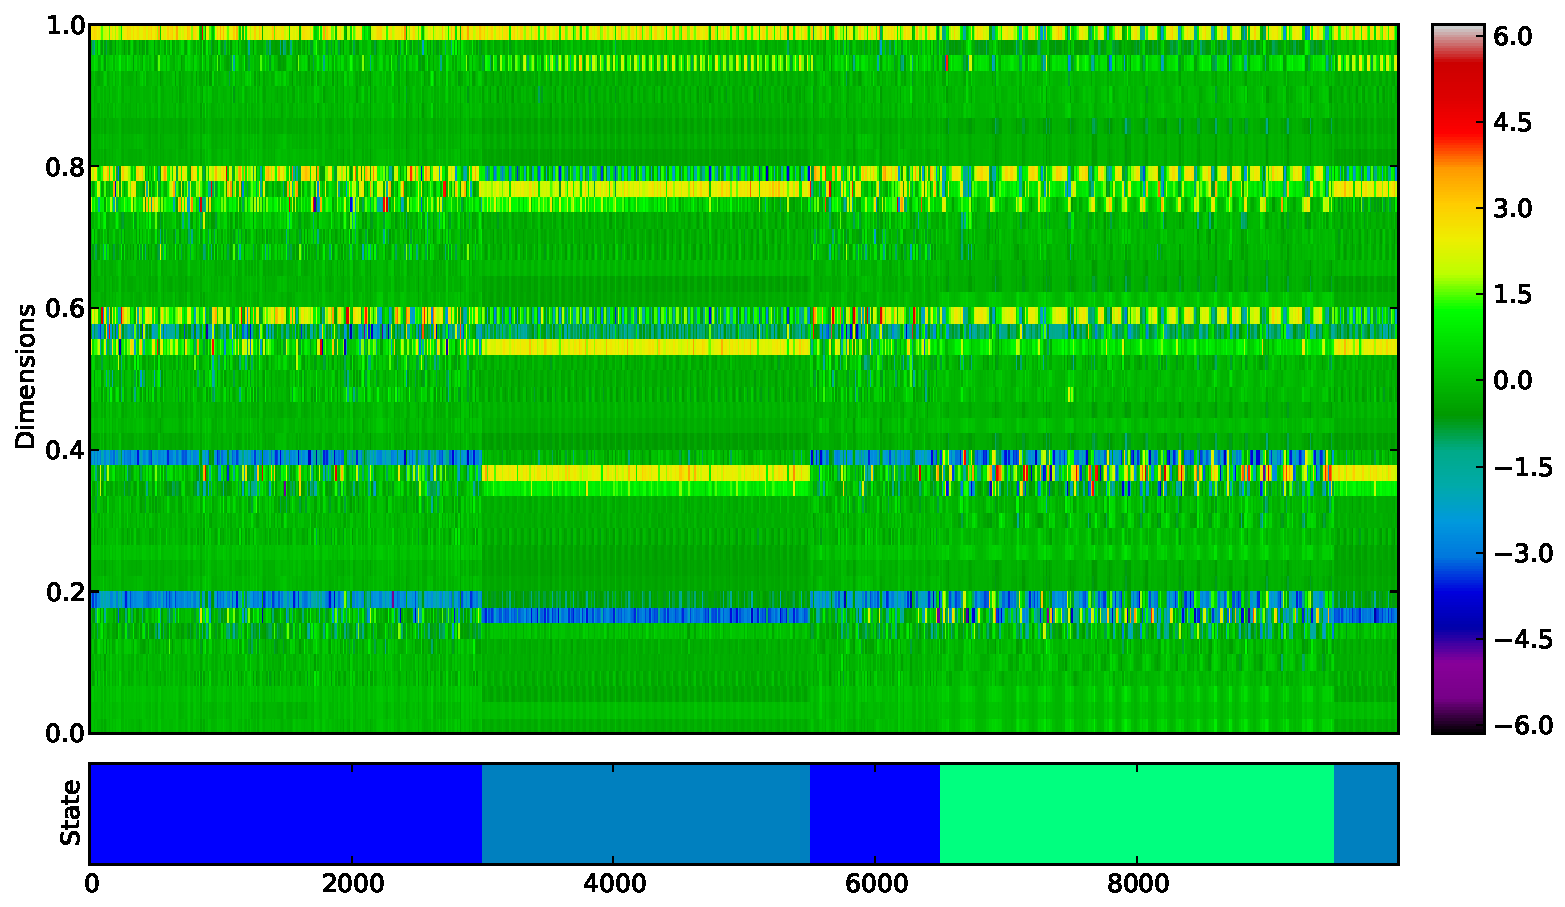
\includegraphics[width=1.\linewidth]{images/accelerometer-data.pdf}
    \label{fig:accelerometer}
\end{figure}

\begin{figure}[htbp]
    \caption{Distribution of Accelerometer Time Series Data.}
  \centering
    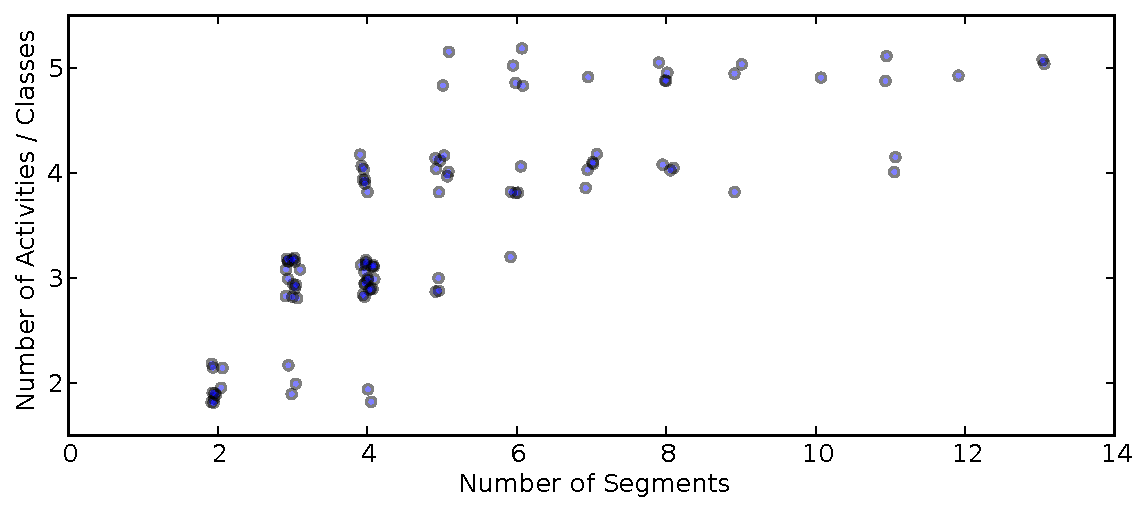
\includegraphics[width=1.\linewidth]{images/distribution_of_dataset_segments.pdf}
    \label{fig:distribution}
\end{figure}

\subsection{Experimental Design}

We compared performance of a standard $K$-state hidden Markov model with our batch-learned regularized HMMs on the two datasets described in the previous section. For the second dataset, we performed a quantitative analysis, treating the task as a multi-class classification problem, and measured the minimum zero-one loss under all possible permutations of output labels, to accommodate the fact that the output labels of an HMM may be a permuted mapping of the true labels. We measured the normalized variation of information~\cite{meila} between the predicted state sequence and true state sequence, which is an information metric capturing the symmetric two-way conditional entropy between two partitionings (clusterings) of a sequence.  In addition to this, we considered the ratio of predicted number of segments to true number of segments, which gives us a sense of whether a method over- or under-segments data, and the absolute segment number ratio (ASNR), which is defined as
\[
    \text{ASNR} = \frac{\max(S_t, S_p)}{\min(S_t, S_p)}
\]
where $S_t$ is the true number of segments in the sequence and $S_p$ is the predicted number of segments. This value tells us how much a segmentation method diverges from the ground truth in terms of relative factor of segments. Lastly, we tracked the number of segments difference between the predicted segmentation and true segmentation and how many segmentations we done perfectly, giving the correct states at all correct positions.

To select parameters for the inertial regularized methods, we used the automated parameter selection procedure discussed in Section~\ref{sec:param-free}. To speed up evaluations, we only ran the automated parameter selection process on ten randomly drawn examples, averaged the final $\zeta$ parameter value, and used the fixed value for all evaluations. The final $\zeta$ parameters are shown in Tables~\ref{tab:results-main} and \ref{tab:results-synthetic}.

We also evaluated the sticky hierarchical Dirichlet process hidden Markov model (HDP-HMM) of Fox \emph{et al.}~\cite{fox2011sticky} on both datasets. The publicly available HDP-HMM toolbox for MATLAB~\cite{HDP-HMM-TOOLKIT} was used, with default settings for the priors. The Gaussian emission model with normal inverse Wishart (NIW) prior were used, and the truncation level $L$ for each example was set to the true number of states, in fairness for comparing with the HMM methods developed here, which are also given the true number of states. The ``stickiness'' $\kappa$ parameter was chosen in a data-driven manner by testing values of $\kappa=0.001$, 0.01, 0.1, 1.0, 5.0, 10.0, 50.0, 100.0, 250.0, 500.0, 750.0 and 1000.0 for best performance over ten randomly selected examples each. The mean performance of the 500th Gibbs sample of ten trials was then taken for each parameter setting, and the best $\kappa$ was empirically chosen. For the synthetic dataset, a final value of $\kappa=10$ was chosen by this method. For the real human accelerometer data, a value of $\kappa=100.0$ provided the best accuracy and relatively strong variation of information performance. These parameter values were used for evaluation on each entire dataset, respectively.

To evaluate the HDP-HMM, we performed five trials one each example in the test dataset, measuring performance of the 1000th Gibbs sample for each trial. The mean performance was then computed for the trials, and the average of all one hundred test examples was recorded.

\section{Results}\label{sec:Results}

\begin{figure}[htbp]
    \caption{Example segmentation of human activities accelerometer data using inertial (MAP) HMM.}
  \centering
    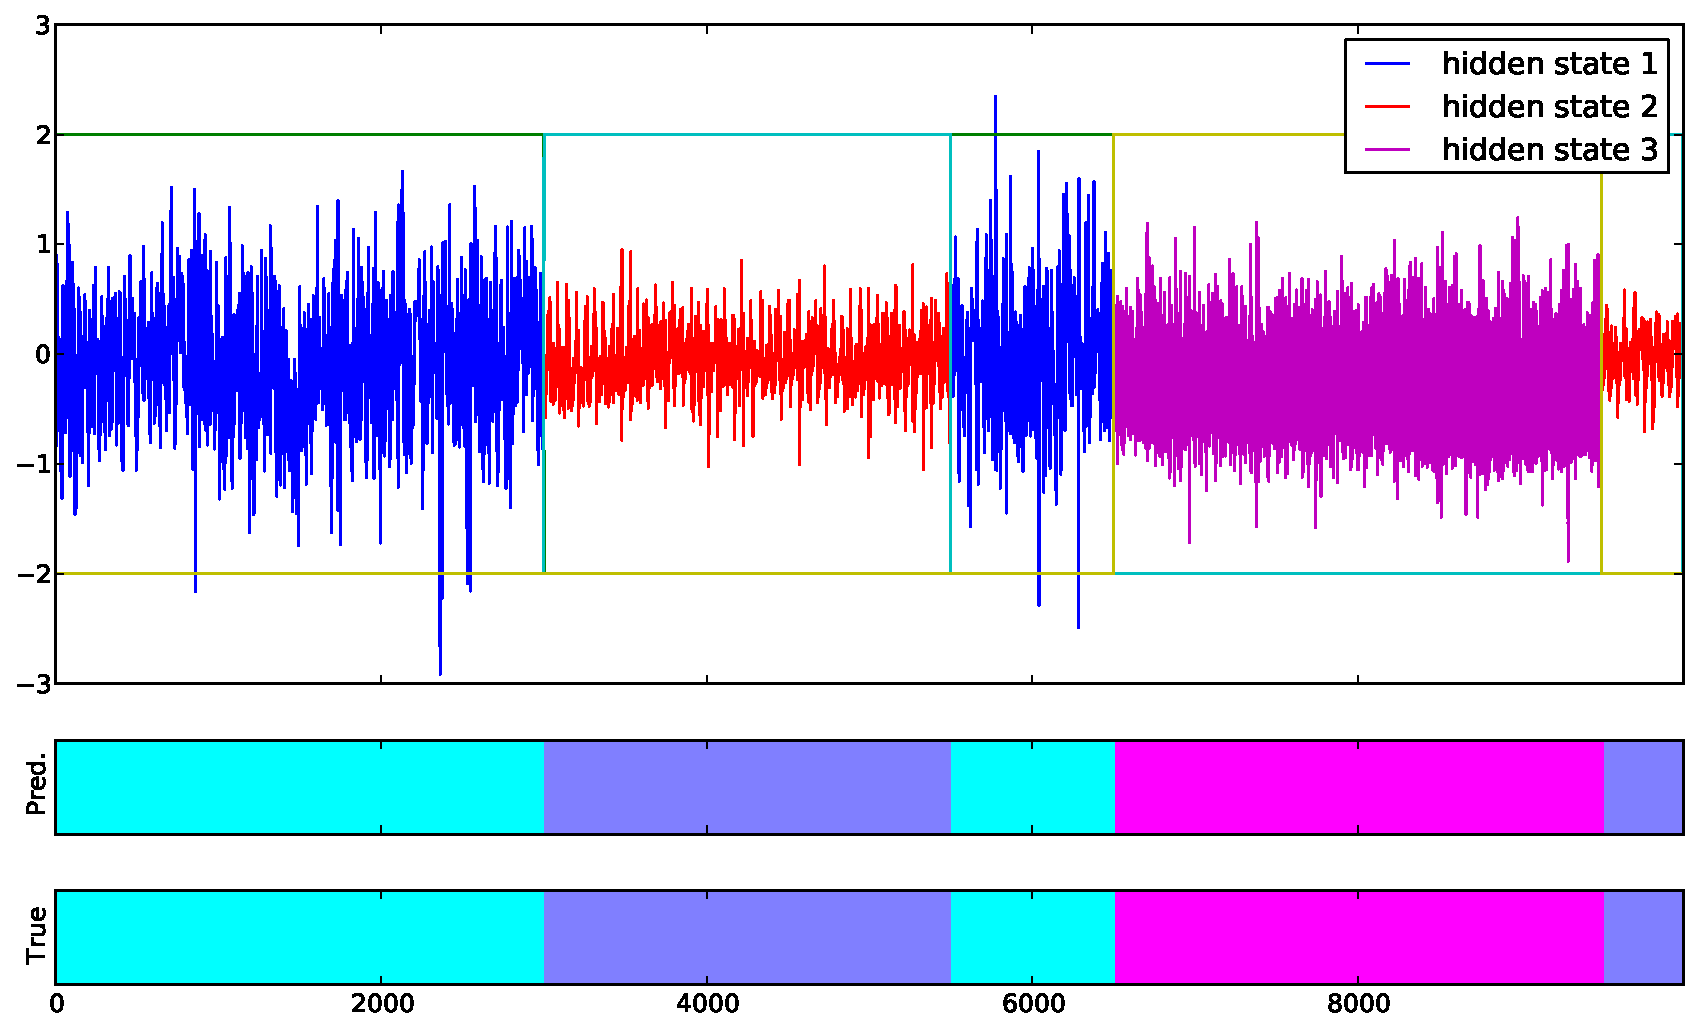
\includegraphics[width=0.8\linewidth]{images/MAP_PARAM_FREE_results_hard_activity_long_1,97_3_states.pdf}
    \label{fig:real-results-MAP}
\end{figure}

\subsection{Synthetic Data Results}
\begin{table}[htbp]
\caption{Results from quantitative evaluation on two-state, 3D synthetic data.}
\resizebox{1.0\linewidth}{!}{
\begin{tabular}{|lrrrrrr|}
\hline
\textbf{Method}                   & \textbf{Accuracy} & \textbf{SNR}  & \textbf{ASNR}     & \textbf{SND}  & \textbf{VOI}    & \textbf{Perfect}  \\ \hline
Sticky HDP-HMM ($\kappa = 10$)    & 0.85              & 0.59          & 3.50              & 2.79          & 0.56            & 0/100                          \\ 
Standard HMM                      & 0.87              & 172.20        & 172.20            & 765.91        & 0.62            & 0/100                          \\ 
MAP HMM ($\zeta = 2.28$)          & 0.99              & 0.96          & 1.13              & 0.51          & 0.07            & 2/100                          \\ 
Inertial PsO HMM ($\zeta = 8.19$) & 0.99              & 0.87          & 1.43              & 1.15          & 0.14            & 1/100                          \\ \hline
\multicolumn{7}{l}{\begin{tabular}[c]{@{}l@{}}
    \vspace{0.05em}\\
    \textbf{Accuracy} = Average Accuracy (value of 1.0 is best)\\ 
    \textbf{SNR} = Average Segment Number Ratio (value of 1.0 is best)\\ 
    \textbf{ASNR} = Average Absolute Segment Number Ratio (value of 1.0 is best)\\ 
    \textbf{SND} = Average Segment Number Difference (value of 0.0 is best)\\ 
    \textbf{VOI} = Average Normalized Variation of Information (value of 0.0 is best)\\ 
    \textbf{Perfect} = Total number of perfect/correct segmentations \end{tabular}} 
\end{tabular}
}
\label{tab:results-synthetic}
\end{table}
Results for the synthetic dataset are shown in Table~\ref{tab:results-synthetic}. Overall, the MAP regularized HMM had the strongest performance, with top scores on all metrics. The inertial pseudo-observation HMM also had strong performance, with extremely high accuracy and low variation of information. The standard HMM suffered from over-segmentation of the data (as reflected in the high SNR, ASNR, and SND scores), while the sticky HDP-HMM tended to under-segment the data. All methods were able to achieve fairly high accuracy on this simple, low-dimensional dataset.

\subsection{Human Activities Accelerometer Data Results}\label{sec:quantitative}
\begin{table}[htbp]
\caption{Results from quantitative evaluation on multivariate human accelerometer data.}
\resizebox{1.0\linewidth}{!}{
\begin{tabular}{|lrrrrrr|}
\hline
\textbf{Method}                   & \textbf{Accuracy} & \textbf{SNR}  & \textbf{ASNR}     & \textbf{SND}  & \textbf{VOI}    & \textbf{Perfect}  \\ \hline
Sticky HDP-HMM ($\kappa = 100$)   & 0.60              & 0.75          &  4.68             & 5.03          & 0.95            & 0/100                           \\ 
Standard HMM                      & 0.79              & 134.59        & 134.59            & 584.16        & 0.38            & 9/100                          \\ 
MAP HMM ($\zeta = 33.5$)          & \textbf{0.94}     & 1.28          & 1.43              & 2.62          & \textbf{0.14}   & \textbf{48/100}                 \\ 
Inertial PsO HMM ($\zeta = 49.0$) & \textbf{0.94}     & \textbf{1.03} & \textbf{1.29}     & \textbf{1.29} & 0.15            & \textbf{48/100}                 \\ \hline
\end{tabular}
}
\label{tab:results-main}
\end{table}

Results from the human accelerometer dataset are shown in Table~\ref{tab:results-main}. Both the MAP HMM and inertial pseudo-observation HMM achieved large gains in performance over the standard HMM model, with average accuracy of 94\%. Furthermore, the number of segments was close to correct on average, with a value near one in both the absolute and simple ratio case. On average, the MAP HMM over-segmented by fewer than three segments, while the inertial pseudo-observation HMM over-segmented by fewer than two on average. Both methods were able to reproduce a perfect segmentation for 48 of the 100 test cases. The average normalized variation of information was low, at $0.14$ and $0.15$ for the MAP and pseudo-observation methods, respectively. Figure~\ref{fig:real-results-MAP} shows the segmentation results for the MAP regularized HMM on a typical sequence, displaying a single dimension of the multivariate time series for clarity. The regularized MAP HMM correctly segments the time series, as can be seen from the congruence between the true and predicted state transition histories (bottom of Figure~\ref{fig:real-results-MAP}).

In comparison, a standard hidden Markov model without inertial regularization achieved accuracy of 79\%, but with average absolute segment number ratio of 134.59 and average normalized variation of information value of $0.38$. On average, the segmentations given by the standard HMM differed by $584.16$ segments, compared to the fewer than three segments difference between the regularized HMMs and the ground truth sequences. The standard HMM was only able to produce perfect segmentations in 9\% of the test cases. Thus, the inertial regularization produces drastic improvements for unsupervised segmentation of human accelerometer activity data.

Even more striking was the improvement over the sticky HDP-HMM of Fox \emph{et al.}~\cite{fox2011sticky}. The performance of that method was poor, with normalized variation of information near 1 (i.e., no correlation between predicted labels and the true segment labels). The method tended to under-segment the data, often collapsing to a single uniform output state. This under-segmentation is reflected in the average segment number ratio (SNR) having a value below one. Problems for this method may have resulted from the moderate dimensionality of the data, an issue suggested by Fox and Sudderth through private correspondence. The sticky HDP-HMM suffers from slow mixing rates as the dimensionality increases, and computation time explodes, being roughly cubic in the dimension. As a result, the one hundred test examples took several days of computation time to complete, whereas the inertial HMM methods took a few hours. 

\section{Discussion}

Our results demonstrate the effectiveness of inertial regularization on HMMs for time series segmentation. Although derived in two independent ways, the MAP regularized and pseudo-observation inertial regularized HMM converge on a similar maximum likelihood update equation, and thus, have similar performance. Either version can be used for segmentation tasks, according to user preference. 

The human activity task highlighted an issue with using standard HMMs for segmentation of time series with infrequent state changes, namely, over-segmentation. Incorporating regularization for state transitions provides a simple solution to this problem. Since our methods rely on changing a single update equation for a standard HMM learning method, they can be easily incorporated into HMM learning libraries with minimal effort. This ease-of-implementation gives a strong advantage over existing persistent-state HMM methods, such as the sticky HDP-HMM framework.

While the sticky HDP-HMM performed moderately well on the low-dimensional synthetic dataset, the default parameters produced poor performance on the real-world accelerometer data. It remains possible that different settings of hyperparameters may improve performance, but the cost of a combinatorial search through hyperparameter space combined with the lengthy computation time of the HDP-HMM method prohibited exhaustive exploration of the space. These results show, at very least, a strong dependence on hyperparameter settings for acceptable performance. In contrast, the inertial HMM methods presented here make use of a simple heuristic for automatically selecting the strength parameter $\zeta$, which resulted in excellent performance on both datasets without the need for hand-tuning several hyperparameters. 

One advantage of the sticky HDP-HMM over the methods presented here is the ability to segment a time series without knowing the number of states beforehand, whereas we require the number of states to be specified for our inertial methods. Thus, while the sticky HDP-HMM has poor performance on the two segmentation tasks, there exists tasks for which the HDP-HMM method is better suited (e.g., when the correct number of states is unknown).

\section{Related Work and Conclusions}

Hidden Markov models for sequential data have enjoyed a long history, gaining popularity as a result of the widely influential tutorial by Rabiner~\cite{rabiner1989tutorial}. Specific to the work presented here, the use of regularization for HMM parameters received a general treatment in~\cite{MAP1994}, for both transition and emission parameters. Our work details a more specific version of the regularization, useful for state persistence. Neukirchen and Rigoll~\cite{neukirchen1999controlling} studied the use of regularization in HMMs for reducing parameter overfitting of emission distributions due to insufficient training data, but without an emphasis on inertial transitioning between states. Similarly, Johnson~\cite{Johnson07whydoesnt} proposed using Dirichlet priors on multinomial hidden Markov models as a means of enforcing sparse emission distributions. 

In contrast, Fox \emph{et al.}\ \cite{fox2011sticky} develop a Bayesian sticky HMM to provide inertial state persistence. They present a method capable of learning a hidden Markov model without specifying the number of states or regularization strength beforehand, using a hierarchical Dirichlet process and truncated Gibbs sampling. Although our method requires the number of states to be specified in advance, their method requires a more complex approach to learning the model and suffers from poor performance for time series with more than ten dimensions. In contrast, our regularization only requires a small change to a single update equation, allowing drop-in regularization for standard Baum-Welch learning algorithms, and performs well on datasets of moderate dimensionality. Furthermore, several hyperparameters for the Bayesian priors must be chosen along with a truncation limit, thus not fully removing the need for specification of parameters, and in fact exacerbating it, since the sticky HDP-HMM requires more parameters than the methods presented here. Our models only require the specification of two parameters, $K$ and $\zeta$, whereas the sticky HDP-HMM requires analogous truncation level $L$ and $\kappa$ parameters to be chosen, in addition to the hyperparameters on the model priors. We have shown that the inertial models are easily implemented, run efficiently, add almost no additional computation effort, and work well on data with over ten dimensions.

Although the methods derived here are simple, they perform well and are computationally efficient. Their simplicity is thus a feature and not a bug. We find that while the two inertial regularization methods differ in derivation and final mathematical form, their performance is similar on the datasets tested, allowing either to be used in practice.  The simplicity of the models thus pave the way for natural modifications and extensions, such as changing the form of the class conditional emission distributions to incorporate internal dynamics. Such extensions are the focus of future work.

\section{Acknowledgments}

The authors would like to thank Emily Fox and Erik Sudderth for their discussions, feedback and assistance with use of the HDP-HMM toolbox.

\bibliographystyle{amsplain}
\bibliography{references}

\end{document}
